
\section{Introduction}
\label{sec:intro}
\begin{figure*}[t!]  % 使用 figure* 让图片跨越两栏
    \centering
    \begin{subfigure}{0.32\textwidth}
        \centering
        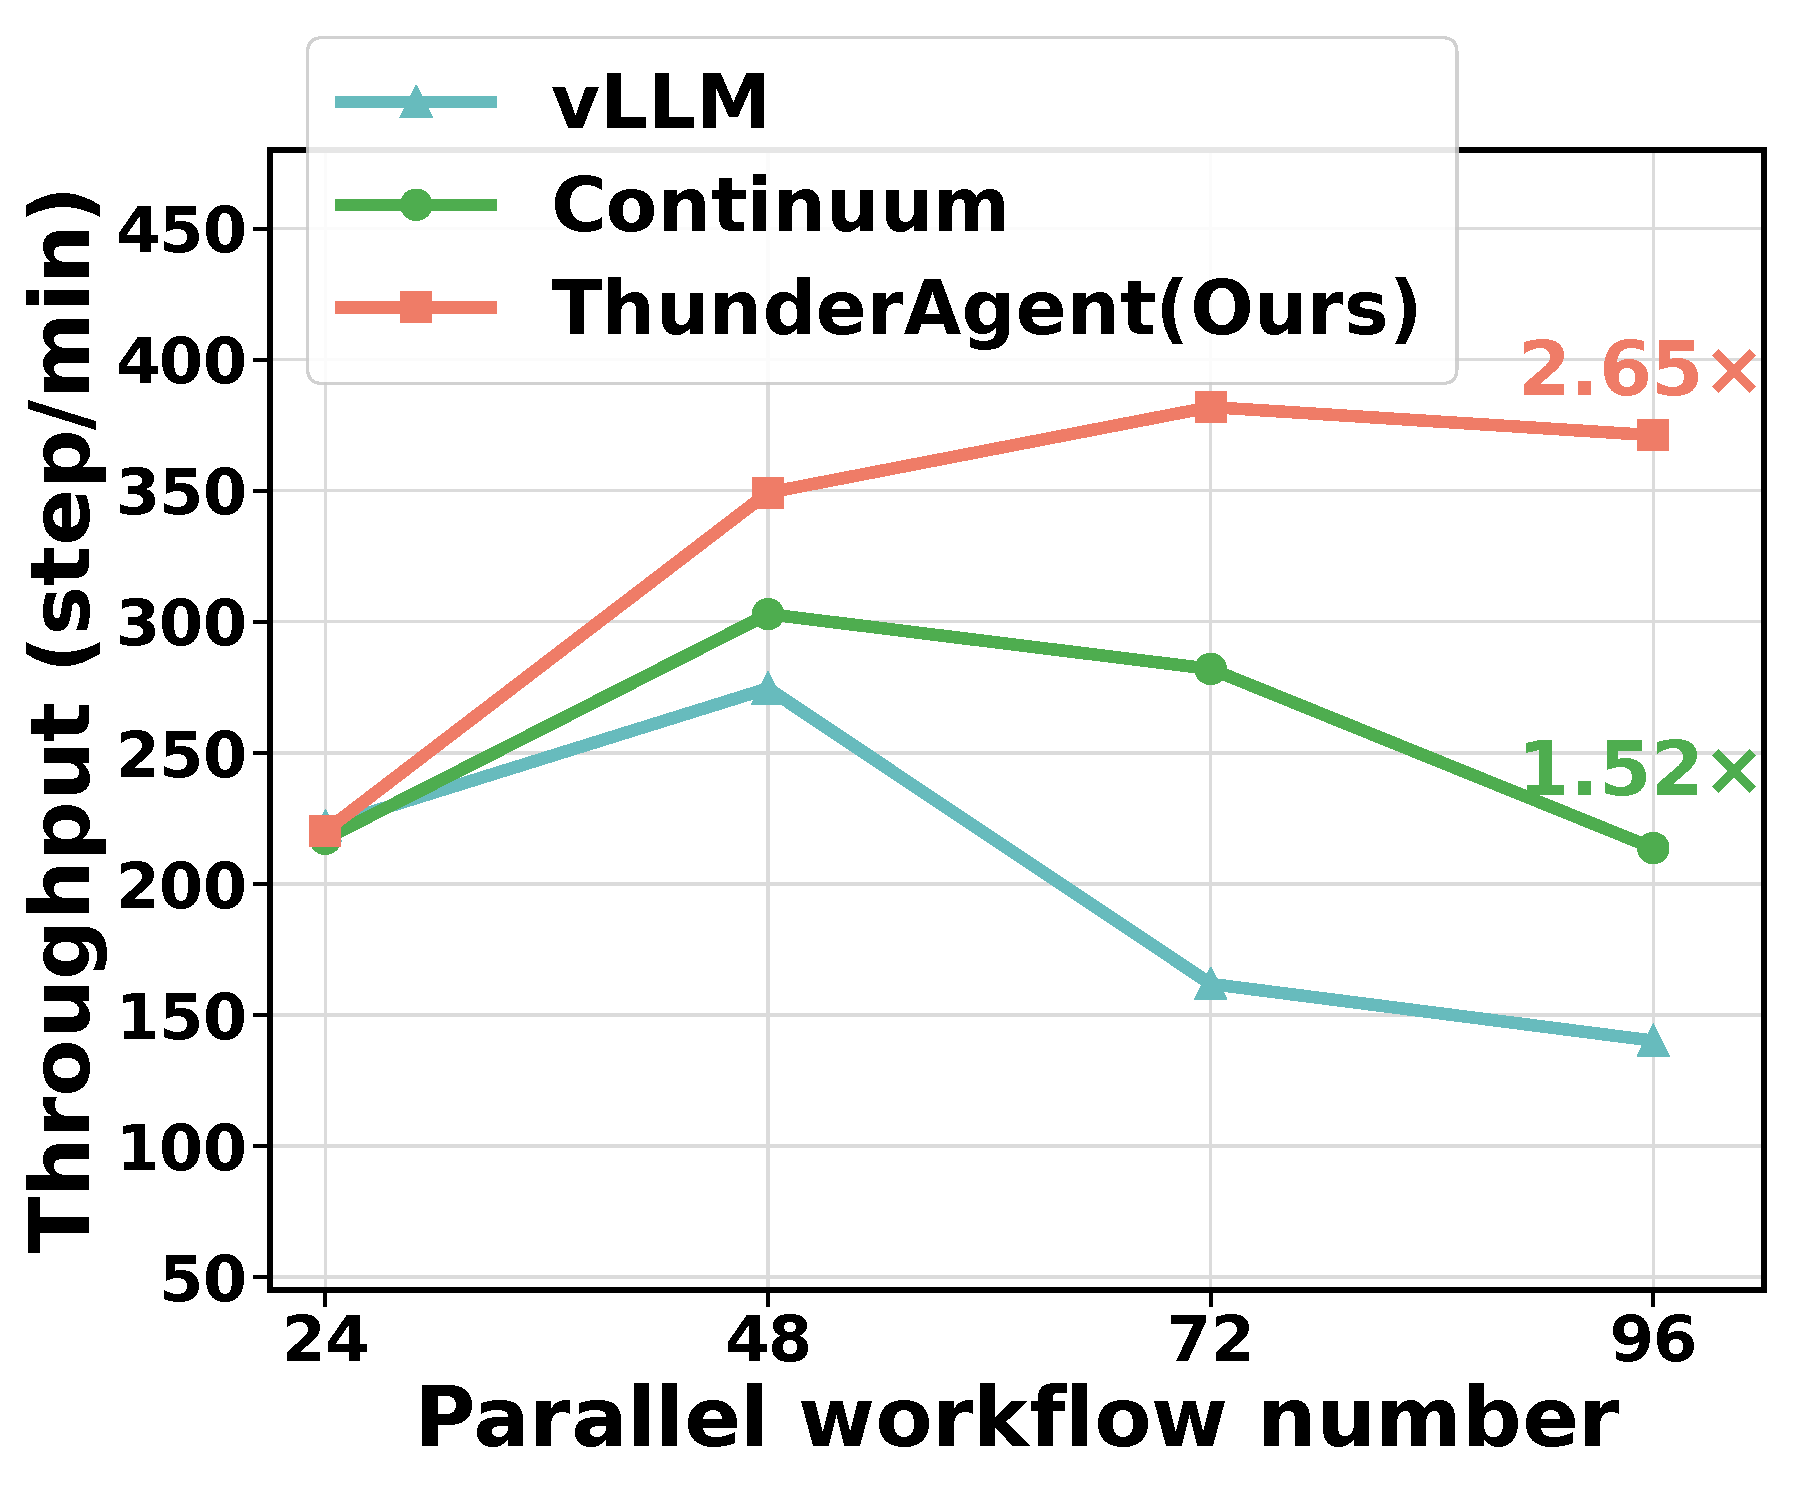
\includegraphics[width=\textwidth]{Figures/throughputs_vs_bs.pdf}  % 替换为你的图片路径
        \caption{Throughput degradation}
        \label{fig:throughputs_vs_bs}
    \end{subfigure}
    \begin{subfigure}{0.32\textwidth}
        \centering
        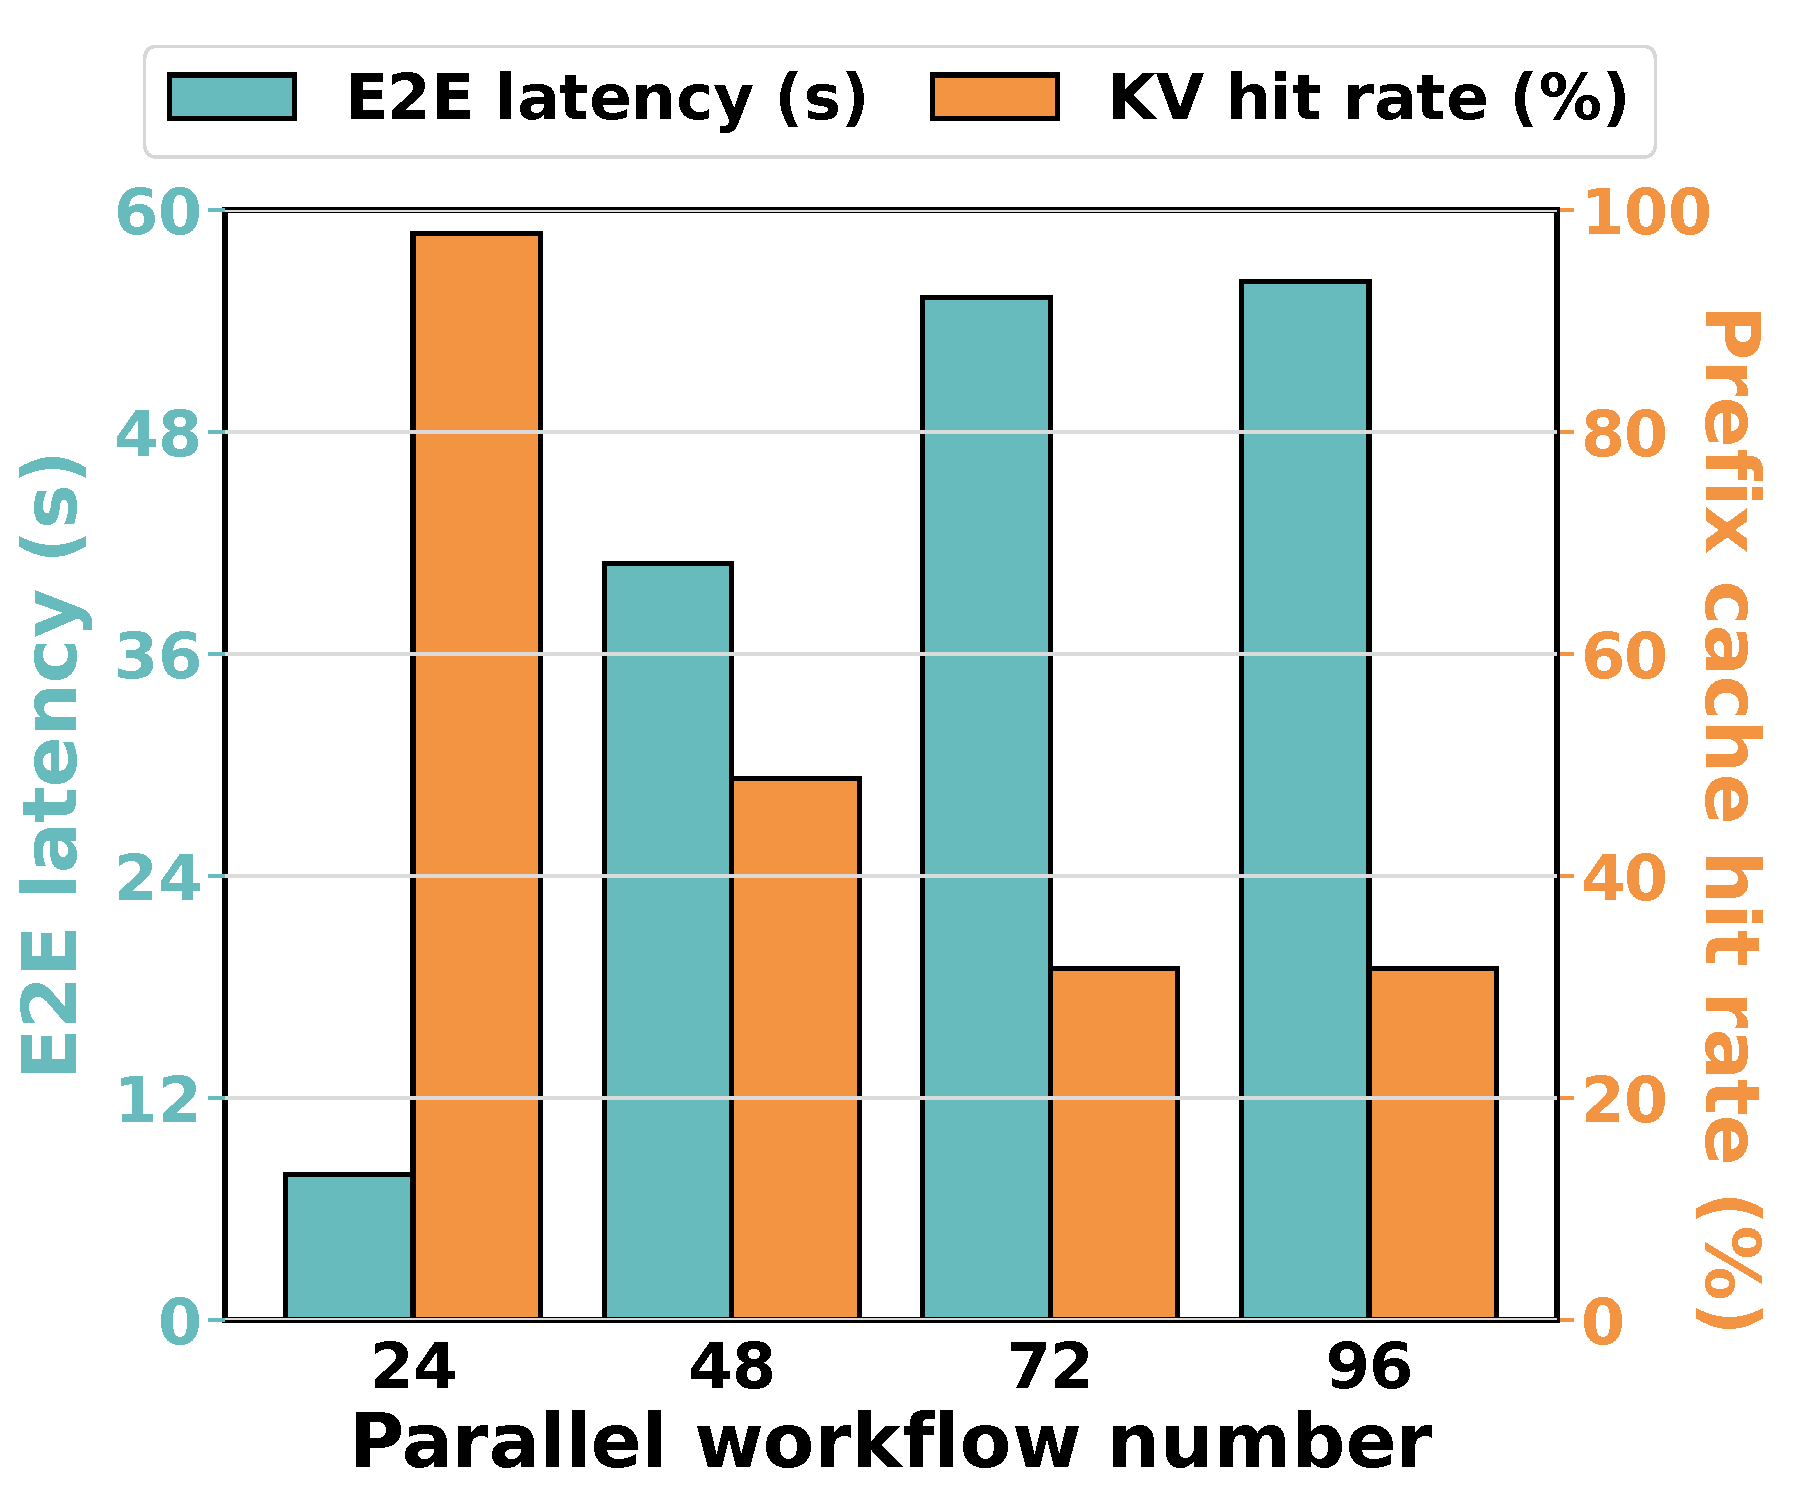
\includegraphics[width=\textwidth]{Figures/cachehit_latency_relation.pdf}  % 替换为你的图片路径
        \caption{KV cache thrashing}
        \label{fig:workload_profile}
    \end{subfigure}
    \begin{subfigure}{0.32\textwidth}
        \centering
        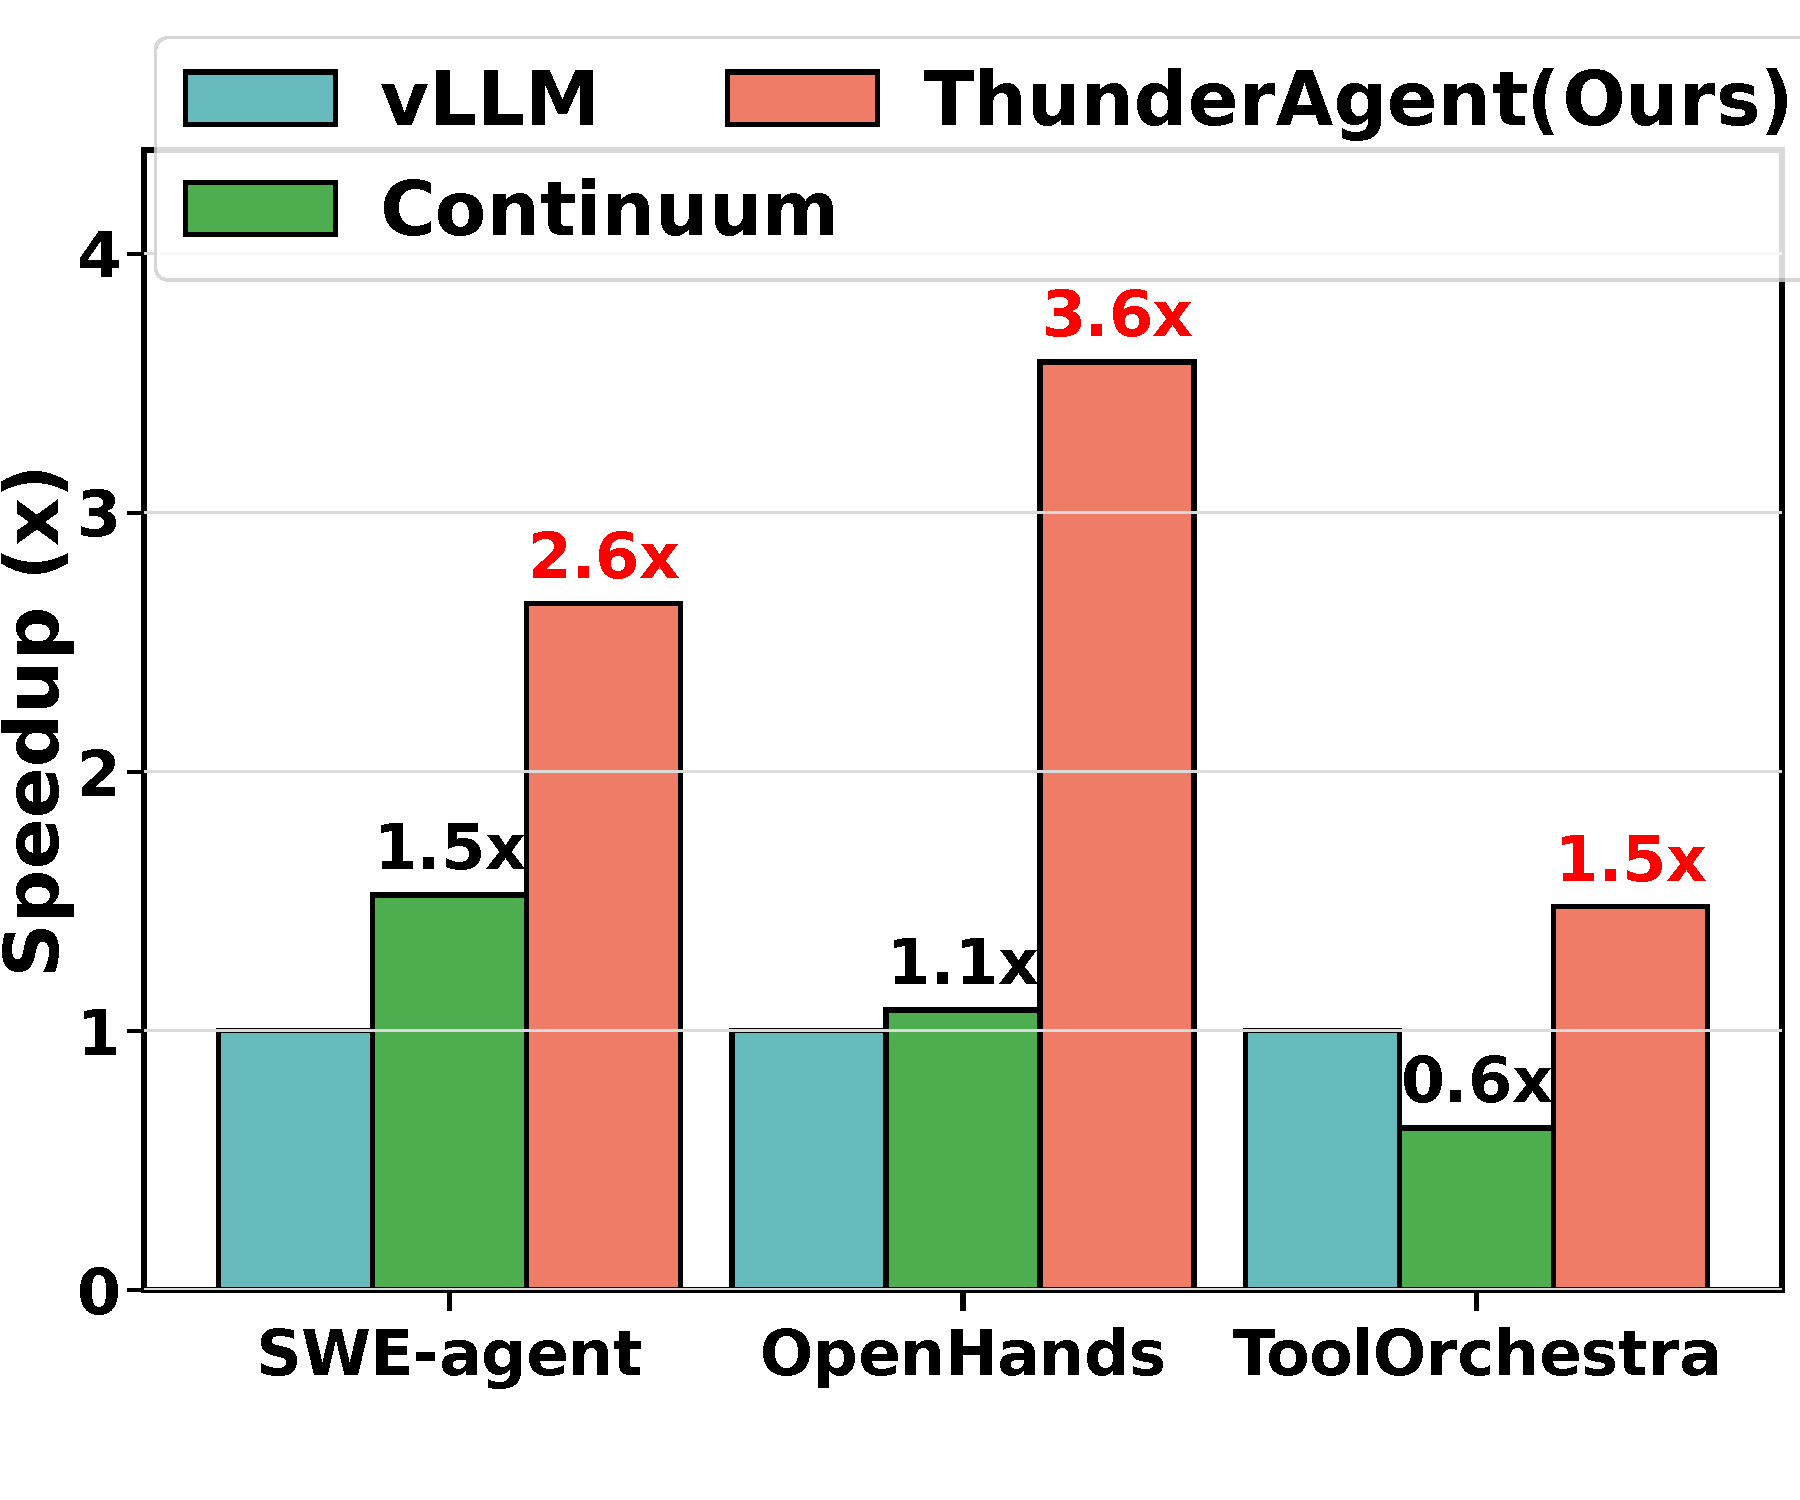
\includegraphics[width=\textwidth]{Figures/throughputs_compare.pdf}  % 替换为你的图片路径
        \caption{ Speedup from \ouralg}
        \label{fig:benefit}
    \end{subfigure}
    \caption{\textbf{Performance comparison of \ouralg against prior agent inference systems as the parallel workflow number (i.e., batch size) increases.} We evaluate the GLM-4.6 MoE model serving SWE-Agent on SWE-Bench Lite (Figures a and b) and SWE-Agent, OpenHands, and ToolOrchestra (Figure c) on an 8$\times$H100 GPU cluster. Results show that: (a) Current inference systems fail to maintain high throughput at large batch sizes. (b) Throughput degradation is primarily caused by low KV cache hit rates, which increase end-to-end request latency. (c) \ouralg achieves high throughput compared to prior inference systems by reducing KV-cache thrashing and managing the lifecycle of tool execution resources.}
    \label{fig:three_subfigures}
    \vspace{-4mm}
\end{figure*}
Recent advances in language models have expanded their use beyond basic chatbots to complex agents~\citep{yang2025qwen3technicalreport, 5team2025glm45agenticreasoningcoding}.
These agents address real-world problems in domains such as coding~\citep{jimenez2024swebenchlanguagemodelsresolve,jain2024livecodebenchholisticcontaminationfree} and computer-use~\citep{xie2024osworldbenchmarkingmultimodalagents,bonatti2024windowsagentarenaevaluating} by interleaving long reasoning with external tool calls (e.g., compilers, retrievers), often operating as
autonomous systems that execute multi-step workflows without real-time human intervention.
However, the throughput of modern inference systems degrades as the number of agentic requests being processed increases (\autoref{fig:throughputs_vs_bs}). Meanwhile, rollout accounts for over \textbf{70\% }of the total wall-clock time in reinforcement learning (RL)~\citep{Sheng_2025, fu2025areallargescaleasynchronousreinforcement}.
% S
% or reinforcement learning rollouts~\citep{hu2024openrlhf, yang2025dashinputawaredynamiclayer}

% Throughput degradation increases the cost and reduces the quality of agent inference systems. Unlike human-in-the-loop systems, where latencies are masked by user response times, agents operate autonomously. Coding and research agents execute long-running trajectories without requiring real-time human intervention. In these non-interactive workflows, maximizing throughput directly reducing the total serving cost by serving with less hardwares. Further, in asynchronous RL frameworks,
% low rollout throughput exacerbates policy lag—the weight discrepancy between training and rollout models, forcing the algorithm to learn from stale data and degrading convergence~\citep{fu2025areallargescaleasynchronousreinforcement, Sheng_2025, shenfeld2025rlsrazoronlinereinforcement,zheng2025stabilizingreinforcementlearningllms}.

As agentic workflows become increasingly autonomous at scale, overall system efficiency is governed by sustained throughput rather than tail latency, whereas human-in-the-loop applications are often dominated by user response times. Therefore, higher throughput directly reduces serving cost by amortizing hardware over more completed workflows. Moreover, in asynchronous RL, higher rollout throughput mitigates policy lag between the parameters used for data collection and those being updated. This allows the model to learn from data with reduced staleness, improving both convergence speed and final policy quality~\citep{fu2025areallargescaleasynchronousreinforcement, Sheng_2025, shenfeld2025rlsrazoronlinereinforcement,zheng2025stabilizingreinforcementlearningllms}.


% The impact is even more severe in agentic reinforcement learning~\citep{hu2024openrlhf, yang2025dashinputawaredynamiclayer}, where rollout relies on extensive interaction with the environment and accounts for over 90\% of the total wall-clock time.
% Crucially, in asynchronous RL frameworks~\citep{fu2025areallargescaleasynchronousreinforcement, Sheng_2025},
% low rollout throughput exacerbates policy lag—the weight discrepancy between training and rollout models, forcing the algorithm to learn from stale data and significantly degrading convergence~\citep{shenfeld2025rlsrazoronlinereinforcement,zheng2025stabilizingreinforcementlearningllms}.

However, current agentic inference systems provide sub-optimal throughput because they are loosely combined from isolated components: an off-the-shelf model inference engine(e.g., vLLM~\citep{kwon2023efficientmemorymanagementlarge} or SGLang~\citep{zheng2024sglangefficientexecutionstructured}) coupled with a general-purpose tool orchestrator (e.g., Kubernetes). While agentic workflows involve multiple turns of model and tool requests, these components schedule and allocate resources separately on a \textit{per-request basis}, without end-to-end knowledge of the entire workflow. This design gives rise to three key challenges:

\begin{enumerate}[itemsep=1pt,topsep=2pt,leftmargin=*]
\item
\textbf{KV cache thrashing.} The request-aware systems prematurely evict KV cache during tool-execution intervals, without foresight into future reuse in the agent workflow.
Thus when the tool call completes, the system needs to rerun prefill to recover its whole interaction history. The re-prefill cost increases the average end-to-end latency of agent workflows by up to \textbf{7.14$\times$} (see \autoref{fig:workload_profile}) and decreases throughput.

\item
\textbf{Cross-node memory imbalance.} The request-aware engines suffer from imbalanced utilization in multi-node inference setups.
% multi-turn agentic trajectories rapidly grow in sequence length causing high GPU memory pressure.
% Typically, routing all requests within a single workload to the same backend yields higher locality.
Existing engines pin all requests from the same agentic workflow to a fixed node to maximize the KV cache hit rate.
However, as context lengths scale rapidly and unpredictably in agent workflows,
% this routing policy leads to memory imbalance across the cluster.
% it lacks the mechanism to transfer active agentic workloads between nodes. Consequently,
% S
some nodes reach capacity while others remain underutilized under this routing policy.

\item
\textbf{Tool lifecycle obliviousness.}
% Most tool resources are shared across all requests within an agentic workload. However,
The request-aware orchestrators struggle to decide when to release and prepare resources and environments required for tool execution.
% lack visibility into the workload lifecycle, these resources are often not released upon task termination.
Thus, unused sandboxes and API servers continue to occupy critical disk space and network ports, leading to cumulative resource exhaustion and system failures.
Meanwhile, agentic workflows have to wait for extremely long setup time before reasoning.
% preparation are usually costly, and these parts could be prepared beforehand to improve end-to-end latency further.
\end{enumerate}

This work introduces \ouralg, an agentic inference system that adopts an end-to-end view of agentic workflows to enable high-throughput agentic serving and RL rollout.
% rather than assembling fragmented request-level components.
% This framework enables the joint orchestration and optimization of LLM inference and tool lifecycles, moving beyond fragmented request-level management.
Our specific contributions are:


% To establish a native serving infrastructure for agentic workflows, we introduce \ouralg, the first system to implement a program-level abstraction with a dedicated scheduler and garbage collector. The program scheduler provides the inference engine with visibility into tool-execution states, mitigating KV-cache thrashing and enabling cross-node program migration to maximize cluster throughput. Simultaneously, the lifecycle-aware garbage collector ensures the timely reclamation of tool resources and enables proactive environment initialization, significantly reducing resource overhead and end-to-end latency.

% \begin{enumerate}[itemsep=0.0pt,topsep=0pt,leftmargin=*]
%   \item \textbf{Program abstraction:} We model agent trajectories as persistent \textit{programs} spanning multiple model/tool steps and exposing semantic state (reasoning/acting/waiting) and resource metadata. This decouples scheduling from execution backends (e.g., vLLM/SGLang, Kubernetes), enabling easy integration of new tasks.

%   \item \textbf{Program-aware scheduler:} We formulate scheduling as constrained optimization to reduce re-prefill overhead and improve decoding throughput under GPU memory limits. We (i) pause tool-acting trajectories during memory pressure to protect reasoning KV cache, and (ii) migrate trajectories across DP nodes via a shared waiting queue to balance memory.

%   \item \textbf{Program-aware tool management:} We overlap I/O-heavy environment setup with LLM reasoning by tracking dependencies, and use termination signals to garbage-collect persistent tool resources (e.g., sandboxes, ports), preventing leaks and sustaining throughput.
% \end{enumerate}

% \junxiong{Is this part too long in abstraction? Should we just keep this a bit more high level, like this 1. We model agent trajectories as persistent \textit{programs} spanning multiple model/tool steps and exposing semantic state (reasoning/acting/waiting) and resource metadata. This decouples scheduling from execution backends (e.g., vLLM/SGLang), enabling easy integration of new tasks. 2. We formulate scheduling as constrained optimization to reduce re-prefill overhead and improve decoding throughput under GPU memory limits. We (i) pause tool-acting trajectories during memory pressure to protect reasoning KV cache, and (ii) migrate trajectories across DP nodes via a shared waiting queue to balance memory. 3. We overlap I/O-heavy environment setup with LLM reasoning by tracking dependencies, and use termination signals to clean up resources, preventing leaks and sustaining throughput.}



\begin{enumerate}[itemsep=0.0pt,topsep=0pt,leftmargin=*]

    \item \textbf{Program abstraction:} We abstract agent workflow as \textit{agentic programs}.
    An agentic program is a first-class scheduling unit that persists across multiple model invocations and tool executions, exposing semantic state to the runtime.
    A program tracks metadata for the workflow's identifier, execution phase  (i.e., reasoning or acting), scheduling status, total tokens, and tool resources. This abstraction decouples scheduling from execution backends (e.g., vLLM/SGLang), enabling seamless integration of new workflows.
    % , and working status (active, paused).

    \item \textbf{Program-aware scheduler:} Based on the program abstraction, we cast agentic inference scheduling as a constrained optimization problem to minimize the recomputation and caching overheads, and maximize prefilling and decoding throughput, subject to GPU memory capacity.
    % We design a program-centric scheduler that utilizes the program metadata to resolve resource contention through
    We introduce two key mechanisms:
    \begin{enumerate}[itemsep=0.0pt,topsep=0pt,leftmargin=*]
        \item \textbf{State-aware pausing:} If the execution backend experiences memory pressure, we selectively pause workflows that are currently in the acting state with tool call. This design helps
        % the scheduler selectively suspends their execution
        preserve memory for programs that are in the reasoning state and eliminate arbitrary, sub-optimal KV cache eviction.
        % that drive KV-cache thrashing.
        \item \textbf{Dynamic migration:} We migrate agent programs across data parallel (DP) GPU nodes to mitigate memory imbalance. We accomplish this by
        % localized memory fragmentation by
        enabling all DP nodes share a global program-aware waiting queue, rather than enforcing that requests from a program are always sent to the same node.
        % Together, these mechanisms prevent systemic bottlenecks and inherently maximize aggregate throughput for both serving and RL rollout.
    \end{enumerate}

    \item \textbf{Program-aware tool resource management:} In long-horizon agentic workloads, tool environments are persistent resources whose mismanagement directly limits sustained throughput. By tracking execution dependencies, \ouralg overlaps I/O-intensive environment initialization with LLM reasoning.
    % , eliminating the idle time caused by serialized bottlenecks.
    For completed programs, we implement a lifecycle-aware garbage collector
    % that bridges the visibility gap between the inference engine and tool managers. By leveraging
    that leverages program termination signals to reclaim tool resources such as Docker sandboxes and network ports.
    % , such as Docker sandboxes and network ports.
    Consequently, this prevents accumulated resource leakage and ensures sustained high-throughput agentic inference in \ouralg.

    % \item \textbf{Extensible Framework and Seamless Integration:} The program-level abstraction provides a unified interface for ReAct-based workflows. By decoupling agent logic from the execution layer, \ouralg enables seamless integration with request-centric backends (e.g., vLLM and SGLang) and orchestrators (e.g., Kubernetes), requiring minimal engineering effort to support new agentic tasks.
\end{enumerate}

The above contributions cannot be achieved within request-aware inference engines. Without an explicit representation of program states and workflow dependencies, request-aware schedulers cannot distinguish temporary tool waits from termination or coordinate GPU memory with program-level resource scheduling.

% We evaluate \ouralg across diverse serving and rollout scenarios, including code agents such as SWE-agent~\citep{yang2024sweagentagentcomputerinterfacesenable} and OpenHands~\citep{wang2025openhandsopenplatformai}, and tool-use agents like ToolOrchestra. Our experiments span SWE-bench~\citep{jimenez2024swebenchlanguagemodelsresolve}, and HLE-bench~\citep{phan2025humanitysexam}, with model scales ranging from 8B Qwen3~\citep{yang2025qwen3technicalreport} to 355B GLM-4.6 MoE~\citep{5team2025glm45agenticreasoningcoding}. Conducted on RTX 5090 and H100 GPU clusters, these evaluations demonstrate that \ouralg achieves \textbf{1.48--3.58$\times$} throughput improvements shown in \autoref{fig:benefit}.

% The program-level abstraction provides a unified interface for ReAct-based workflows.
We evaluate \ouralg across diverse agentic workloads. For \textbf{serving}, we evaluate the ToolOrchestra~\citep{su2025toolorchestraelevatingintelligenceefficient} as routing agent on HLE-Bench~\citep{phan2025humanitysexam}, SWE-Agent~\citep{yang2024sweagentagentcomputerinterfacesenable} and OpenHands~\citep{wang2025openhandsopenplatformai} as coding agent on SWE-bench~\citep{jimenez2024swebenchlanguagemodelsresolve}, and OpenHands as scientific discovery agent on ScienceAgentBench~\citep{chen2024scienceagentbenchrigorousassessmentlanguage}, achieving \textbf{1.48--3.58$\times$} throughput improvements as illustrated in \autoref{fig:benefit}. For \textbf{RL rollouts}, we further test the coding agents on distributed GPU nodes, achieving  \textbf{1.79--3.92$\times$} improvements compared with prior SOTA systems.

% We evaluate \ouralg across diverse agentic workloads, including \textbf{RL rollouts and serving} for coding agents such as SWE-Agent~\citep{yang2024sweagentagentcomputerinterfacesenable} and OpenHands~\citep{wang2025openhandsopenplatformai}, alongside \textbf{standard serving} for tool-use agents like ToolOrchestra~\citep{su2025toolorchestraelevatingintelligenceefficient}. Our experiments span SWE-bench~\citep{jimenez2024swebenchlanguagemodelsresolve} and HLE-bench~\citep{phan2025humanitysexam}, with model scales ranging from 8B Qwen3~\citep{yang2025qwen3technicalreport} to 355B GLM-4.6 MoE~\citep{5team2025glm45agenticreasoningcoding}. We conduct experiments on RTX 5090 and H100 GPU clusters, demonstrating that \ouralg achieves \textbf{1.48--3.58$\times$} throughput improvements across settings, shown in \autoref{fig:benefit}.

% We also implemented our system at a leading ai inference company to speed up their coding agent RL training workload by \textbf{2.31$\times$} in total.


% However, current agent serving systems are not designed to satisfy such throughput demands.

% Most agentic serving frameworks are constructed by assembling independent resource management tools, typically coupling request-level serving engines like vLLM~\citep{kwon2023efficientmemorymanagementlarge} and SGLang~\citep{zheng2024sglangefficientexecutionstructured} with general-purpose tool schedulers like Kubernetes. This architecture presents a granularity misalignment: serving engines are optimized for stateless, independent requests, utilizing KV-cache eviction policies like Least Recently Used (LRU) to maximize instantaneous GPU utilization. Consequently, these systems treat the interval of external tool execution as a session termination or generic idleness, ignoring the agent's requirement to persist context for subsequent steps. This leads to premature KV-cache eviction: when the tool execution concludes, the system is forced to re-prefill the full history, leading to massive cache misses and causing significant computational overhead. \autoref{fig:workload_profile} shows that request-level infrastructures failed to maintain high throughputs in large batch serving due to heavy re-prefill latency. While recent schedulers like Continuum~\citep{li2025continuumefficientrobustmultiturn} attempt to address this via predictive pinning, they rely on the assumption of deterministic tool durations. In agentic workflows like Tool Orchestra~\citep {su2025toolorchestraelevatingintelligenceefficient} and GPU Kernel Scientist~\citep{andrews2025gpukernelscientistllmdriven} that interact with complex environments, however, tool execution times are inherently variable, making prediction-based mechanisms difficult to stabilize in practice.

% \yinfang{I like this paragraph, but it can be written better by providing more details.}



% Furthermore, the absence of a unified program abstraction prevents the coordinated management of heterogeneous resource lifecycles under stochastic workloads. Specifically, the lifecycle of the GPU resource operates independently from its tools and environment (Docker/Sandbox). This disjoint management leads to inefficient resource reclamation, where "zombie" tools like sandboxes persist in memory and disk after an agent has finished or stalled, limiting the scheduling of new tasks.

% Large Language Models (LLMs) have demonstrated exceptional performance in single-turn generation tasks, such as mathematical reasoning and question answering.
% However, solving composite real-world problems requires extending these capabilities to multi-turn interactions, where the model must maintain persistent context across extended sessions.
% This paradigm is further expanded in agentic workflows.
% Notably, the ReAct framework has emerged as the \textit{de facto} standard for constructing such systems.
% By interleaving multi-step reasoning with the execution of \textbf{heterogeneous external tools}, such as compilers, terminals, and remote APIs, ReAct agents can autonomously accomplish composite tasks[cite: 4, 10].

% However, this transition comes with an throughputs Degradation on infrastructure. Executing these long-lived, multi-turn programs consumes vast inference budgets, not just in GPU compute and memory, but across heterogeneous resources including costly remote model APIs, CPU and disk I/O for sandbox and retriever.
% Our empirical analysis reveals a startling gap: compared to single-turn code generation benchmarks BigCode Bench, running multi-turn agentic workloads, Openhands, results in over \textbf{9.7$\times$ throughput degradation} and consumes massive storage, over \textbf{6TB} of disk usage in our large-scale stress tests.

% This throughput degradation constitutes a fundamental bottleneck for autonomous agentic systems.
% Unlike human-in-the-loop applications, where system latency is masked by user response time, agents operate continuously and autonomously.
% Consequently, system throughput directly dictates the feasibility of large-scale evaluation(e.g., running SWE-bench on thousands of instances) and the cost-efficiency of deployment[cite: 7, 8].
% This bottleneck is even more pronounced in Agentic Reinforcement Learning (RL), where rollout relies on extensive interaction with the environment.
% Studies indicate that this rollout phase dominates the training budget, accounting for over 83\% of the total wall-clock time.

% Crucially, in asynchronous RL frameworks, low rollout throughput exacerbates the latency between data generation and model updates, increasing the divergence between the rollout policy and the training policy (policy lag).
% Thus, maintaining high throughput of large batch serving and rollout is a prerequisite for both efficient serving and stable RL training.


% Crucially, in asynchronous training frameworks, low rollout throughput exacerbates the "policy lag"—the weight difference between the training model and the rollout model. This latency forces the algorithm to learn from stale, off-policy data, significantly degrading convergence speed and accuracy. Thus, maintaining high throughput in large-batch scenarios is a prerequisite for effective Agentic RL.

% Current infrastructure is not designed to satisfy agentic throughput demands.
% Most agentic serving frameworks are constructed by assembling independent resource management tools, typically coupling request-level serving engines (e.g., vLLM, SGLang) with general-purpose tool schedulers (e.g., Kubernetes, retriever server).


% This architecture presents a \textbf{granularity misalignment}: serving engines are optimized for stateless, independent requests, utilizing KV cache eviction policies like Least Recently Used (LRU) to maximize instantaneous GPU utilization.
% Consequently, these systems treat the interval of external tool execution as a session termination or generic idleness, ignoring the agent's requirement to persist context for subsequent steps.
% This leads to premature KV-cache eviction: when the tool execution concludes, the system is forced to re-pefill the full history, leading to huge KV cache missrate and causing significant computational overhead and throughput degradation[cite: 36, 41, 42].

% Furthermore, this lack of a unified program-level view fail to manage the \textbf{coupled lifecycles} of heterogeneous resources in the face of workload stochasticity.
% Specifically, the lifecycle of the GPU resource operates independently from its tools and environment (Docker/Sandbox).
% This disjoint management could lead to unefficient garbage collection, where sandboxes persist in memory and disk after an agent has finished or stalled—limiting the scheduling of new tasks.
% While recent schedulers like Continuum address preemption via predictive pinning, they rely on the assumption of deterministic tool durations. However, pinned KV caches could still be evicted in extreme heavy workloads. And in complex agentic workflows, tool execution times are inherently variable (e.g., dependent on network I/O or search depth), making such prediction-based mechanisms difficult to stabilize in practice.

% Furthermore, this lack of a unified program-level view affects heterogeneous resource orchestration.
% In current systems, the lifecycle of the GPU resource operates independently from its tool and environment (Docker/Sandbox).
% This separation often leads to \textbf{"Zombie" containers}—where sandboxes persist in memory and disk after an agent has finished or stalled—limiting the scheduling of new tasks.
% While recent schedulers like Continuum address this via predictive pinning, they assume deterministic tool durations.
% However, in complex agentic workflows, tool execution times are variable, making prediction-based pinning difficult to stabilize in practice.

% To bridge this gap, we present \textbf{ThunderReact}, a program-centric infrastructure designed specifically for the efficient serving and rollout of stateful agentic systems. Unlike prior works that optimize components in isolation, ThunderReact treats the agent program as the first-class scheduling entity, orchestrating the end-to-end lifecycle of both neural and symbolic resources. Through our experiments on various agent tasks and models, our method have show no throughput degradation in large batch serving and rollout with 3$\times$ improvements compared with request level serving engine and 4$\times$ disk memory saving with tool optimizations. Our specific contributions are:

% \begin{itemize}
%     \item \textbf{Program-Centric Abstraction and Infrastructure:} We formalize the agentic task as a program, a continuous scheduling entity that encapsulates both GPU and other heterogeneous resources. Based on this abstraction, we architect a unified infrastructure designed to synergistically optimize the execution of complex agentic tasks. By implementing a feedback-based congestion control mechanism that minimizes the \textit{Resource-Time Product}[cite: 89, 91], our system maintains high throughputs and is cost-efficient for agentic serving and rollout.

%     \item \textbf{Multi-Node Program-Level Scheduler:} We design a distributed scheduler to address memory imbalance and preemption challenges in multi-node serving and rollout. By tracking the memory footprint and execution stage of each program, our system transforms rigid load balancing (or simple KV-aware routing) into \textbf{dynamic stateful placement}. This mechanism enables \textbf{collaborative preemption and active migration}, where programs on congested nodes are proactively paused and moved to underutilized workers. This dynamic re-balancing effectively resolves hot-spots and prevents head-of-line blocking caused by long-context agents.

%     \item \textbf{Lifecycle-Coupled Resource Optimization:} We implement fine-grained resource management for heterogeneous tools, featuring program-aware garbage collection and request-level micro-batching[cite: 147, 149]. By coupling the lifecycle of Docker sandboxes with the agent program, we ensure immediate resource reclamation upon task completion. Furthermore, our micro-batching strategy for tool execution mitigates I/O contention during large-batch rollouts, preventing system overload from concurrent external requests.
% \end{itemize}





% 1. LLM agents are transfering single turn generation to multiple generations with tool call. (Introduce react agent, \textbf{single turn -> multiturn turn -> multiturn with outside multiple resource}) Do we need a figure of react agent? We do not need it just use words to describe. An example figure
% % \textbf{显示不是单一LLM而是多方面的tools}
% 2. These agents are very expensive in evaluate and rollout. (figure 1 here, x-axis parallel task number?, y-axis average program execution time with prefill/decode/tool call ratio). \textbf{One sentence is enough, there is no need to put a graph} No figure here.

% 3. In such senarios, throughputs is the most important figure for efficiency. Current request level serving engine vllm. sglang failed to work well at large batch evaluation RL. (figure 1 here, x-axis is parallel task number, y-axis is throughput(step/min? token/s?))
% % \textbf{现在serving engine没有考虑programing level的关系，问题出在很多层面比如disk/cpu/GPU一个最主要的例子是GPU memory contention}
% 4. This is because KV cache is program level resource. multiturn task will preempt each other and make kv hit rate really slow and cause reprefill. (Figure3 here, x-axis parallel task number, y-axis KV cache hit rate)
% % Hetergenious system, 管理LLM，管理tool，管理所有事情。强调Disk usage，要讲的大一点，vllm + program没办法解决全部的问题。

% 4. Our contribution
%     1) Program level congestion control
%     2) multinode program-level scheduler
%     3) program-level outside reousce life cycle control and large batch optimization.